%%%%%%%%%%%%%%%%%%%%%%%%%%%%%%%%%%%%%%%%%%%%%%%%%%%%%%
% Thanks to Xu Minghao's work                        %
% I modify it into uchicago version                  %
% to not make new bug, I don't alter "Ritsumeikan"   %
% keywords in file. Pls feel free to use             %
%%%%%%%%%%%%%%%%%%%%%%%%%%%%%%%%%%%%%%%%%%%%%%%%%%%%%%

%%%%%%%%%%%%%%%%%%%%%%%%%%%%%%%%%%%%%%%%%%%%%%%%%%%%%%
% A Beamer template for Ritsumeikan University       %
% Author: Ming-Hao Xu (Xu Minghao)                   %
% Date:   April 2022.                                %
% LPPL Licensed.                                     %
%%%%%%%%%%%%%%%%%%%%%%%%%%%%%%%%%%%%%%%%%%%%%%%%%%%%%%

\documentclass[spanish]{beamer}
\usepackage{Ritsumeikan}
\usepackage[export]{adjustbox}
\usepackage{hyperref}
\usepackage[T1]{fontenc}
\usepackage[backend=bibtex,style=ieee,maxnames=1,minnames=1]{biblatex}
\addbibresource{ref.bib}
% other packages
\usepackage{latexsym,amsmath,xcolor,multicol,booktabs,calligra}
\usepackage{graphicx,pstricks,listings,stackengine}
\usepackage{tikz}
\usepackage{media9}
\usepackage{multimedia}
% dummy text; remove it when working on this template
\usepackage{lipsum}
%Language Packages
\usepackage[spanish]{babel}
\usepackage{ragged2e}
\justifying%

% Definir nuevos comandos para los integrantes y la facultad
\author[Carrillo B. José E. \&  Robles O. José A.]{Carrillo Barreiro José Emiliano \\ Robles Ortero José Ángel}
\title{Trabajo Terminal No. 2025-B065}
\subtitle{Modelo para representar la interacción gravitacional de dos cuerpos}
\institute{Instituto Politécnico Nacional \\ Escuela Superior de Cómputo}
\newcommand{\directortesis}{Dr.\ Cesar Hernández Vasquez}
\newcommand{\codirectortesis}{Dr.\ Mauricio Olguín Carbajal}
\date{\today}

% defs
\def\cmd#1{\texttt{\color{red}\footnotesize $\backslash$#1}}
\def\env#1{\texttt{\color{blue}\footnotesize #1}}
\definecolor{deepblue}{rgb}{0,0,0.5}
\definecolor{ccnuMainColor}{RGB}{0,86,109}
\definecolor{deepgreen}{rgb}{0,0.5,0}
\definecolor{halfgray}{gray}{0.55}

\lstset{
    basicstyle=\ttfamily\small,
    keywordstyle=\bfseries\color{deepblue},
    emphstyle=\ttfamily\color{ccnuMainColor},    % Custom highlighting style
    stringstyle=\color{deepgreen},
    numbers=left,
    numberstyle=\small\color{halfgray},
    rulesepcolor=\color{red!20!green!20!blue!20},
    frame=shadowbox,
}


\begin{document}

    \begin{frame}
        \titlepage%
    \end{frame}

    \include{secciones/01-introduccion}
    \section{Estado del Arte}

\begin{frame}{Estado del arte}
    \centering
    \captionof{table}{Comparativa contra soluciones disponibles}%
    \label{tab:arte}
    \vspace{-0.1cm}
    \begin{adjustbox}{max width=0.9\textwidth,max height=0.7\textheight, keepaspectratio}
        \renewcommand{\arraystretch}{1.3}
            \begin{tabular}{@{}>{\bfseries}p{0.35\textwidth} p{0.4\textwidth} p{0.20\textwidth} p{0.15\textwidth} p{0.35\textwidth}@{}}
            \toprule
            \textbf{Producto o metodo} & \textbf{Características} & \textbf{Escalabilidad} & \textbf{Usa IA} & \textbf{Cambios dinamicos} \\
            \midrule
            ode\_num\_int & Framework C++11 modular para EDOs; orientado a pruebas de integradores. & Media & No & No \\
            Representación Geométrica & Quadtrees/Octrees para geometría eficiente, no simula dinámica. & Alta & No & No \\
            Método n-NNN & Simulación con n-vecinos y cirugía Hamiltoniana; inspirado en IA. & Alta & Sí & No \\
            PKDGRAV3 & Hidrodinámica sin malla (MFM/MFV); vecinos adaptativos. & Alta & No & No \\
            \bottomrule
            \end{tabular}
    \end{adjustbox}
    \smallskip
\end{frame}



\begin{frame}{Estado del arte}
    \centering
    \captionof{table}{Comparativa contra soluciones disponibles}%
    \label{tab:arte}
    \vspace{-0.1cm}
    \begin{adjustbox}{max width=0.9\textwidth,max height=0.7\textheight, keepaspectratio}
        \renewcommand{\arraystretch}{1.3}
            \begin{tabular}{@{}>{\bfseries}p{0.35\textwidth} p{0.4\textwidth} p{0.20\textwidth} p{0.15\textwidth} p{0.35\textwidth}@{}}
            \toprule
            \textbf{Producto o metodo} & \textbf{Características} & \textbf{Escalabilidad} & \textbf{Usa IA} & \textbf{Cambios dinamicos} \\
            \midrule
            SPH/N-body Híbrido & Interacciones gas-estrella con árbol Barnes-Hut y pasos bloque. & Alta & No & No \\
            Integrador Simpléctico & Orden 2+, reversible; ideal para colisiones. & Media & No & No \\
            Solver TPM & Combina PM y Tree según densidad local; altamente paralelizado. & Alta & No & No \\
            Algoritmo TPM & Descomposición por densidad; integración multi-escala. & Alta & No & No \\
            \bottomrule
            \end{tabular}
    \end{adjustbox}
    \smallskip
\end{frame}


\begin{frame}{Estado del arte}
    \centering
    \captionof{table}{Comparativa contra soluciones disponibles}%
    \label{tab:arte}
    \vspace{-0.1cm}
    \begin{adjustbox}{max width=0.9\textwidth,max height=0.7\textheight, keepaspectratio}
        \renewcommand{\arraystretch}{1.3}
            \begin{tabular}{@{}>{\bfseries}p{0.35\textwidth} p{0.4\textwidth} p{0.20\textwidth} p{0.15\textwidth} p{0.35\textwidth}@{}}
            \toprule
            \textbf{Producto o metodo} & \textbf{Características} & \textbf{Escalabilidad} & \textbf{Usa IA} & \textbf{Cambios dinamicos} \\
            \midrule
            REBOUND & Modular; incluye varios integradores, colisiones y condiciones frontera. & Alta & No & No \\
            Estabilidad Planetaria & Estudio con REBOUND; Gini vs. inestabilidad. No eventos internos. & Alta & No & No \\
            \midrule
            \rowcolor{yellow!20}
            \textbf{Solución Propuesta} & \textbf{Combina FMM/Barnes-Hut para cálculo gravitacional eficiente con Algoritmos Bioinspirados para la \textit{optimización y ajuste dinámico} de parámetros (masa) durante la simulación.}  & \textbf{Alta} & \textbf{SÍ} & \textbf{SÍ} \\
            \bottomrule
            \end{tabular}
    \end{adjustbox}
    \smallskip
\end{frame}

    \section{Marco Teórico}
\subsection[Tecnologías]{Tecnologías: Lenguaje \& Librerias.}

\begin{frame}{Lenguaje de Programación}{Python}
    \begin{columns}
        \begin{column}{0.4\textwidth}
            % Aquí podrías incluir una imagen de ejemplo
            \centering
            \begin{figure}[H]
                \centering
                \adjustbox{max width=\textwidth, max height=0.5\textheight}{%
                
\includegraphics{img/marcoTeorico/python-logo.png}
                }
                \vspace{-0.25cm}
                \caption{\tiny~Logo de Python \textit{Adaptado de:}~\cite{PythonSoftwareFoundation}}%
                \label{fig:Python_logo}
            \end{figure}
        \end{column}
        \begin{column}{0.6\textwidth}
            \begin{itemize}
                \item Alto nivel y propósito general
                \item Sintaxis clara
                \item Multiparadigma
                \item Tipado dinámico
                \item Extensa biblioteca
            \end{itemize}
        \end{column}
    \end{columns}
\end{frame}

\begin{frame}{Biblioteca de Simulación N-Cuerpos}{REBOUND}
    \begin{columns}
        \begin{column}{0.6\textwidth}
            \begin{itemize}
                \item Implementado en C
                \item Dinámica colisional y no colisional
                \item Integradores avanzados
                \item Algoritmos de gravedad
                \item Detección y resolución de colisiones
            \end{itemize}
        \end{column}
        \begin{column}{0.4\textwidth}
            % Aquí podrías incluir una imagen de ejemplo
            \centering
            \begin{figure}[H]
                \centering
                \adjustbox{max width=1.4\textwidth, max height=0.5\textheight}{%
                
\includegraphics{img/marcoTeorico/reboundblack-logo.png}
                }
                \vspace{-0.25cm}
                \caption{\tiny~Logo de REBOUND \textit{Adaptado de:}~\cite{Rein2012}}%
                \label{fig:REBOUND_logo}
            \end{figure}
        \end{column}
    \end{columns}
\end{frame}

\begin{frame}{Biblioteca de Optimización}{pymoo}
    \begin{columns}
        \begin{column}{0.4\textwidth}
            % Aquí podrías incluir una imagen de ejemplo
            \centering
            \begin{figure}[H]
                \centering
                \adjustbox{max width=\textwidth, max height=0.5\textheight}{%
                
\includegraphics{img/marcoTeorico/pymoo-logo.png}
                }
                \vspace{-0.25cm}
                \caption{\tiny~Logo de pymoo \textit{Adaptado de:}~\cite{blank2020}}%
                \label{fig:pymoo_logo}
            \end{figure}
        \end{column}
        \begin{column}{0.6\textwidth}
            \begin{itemize}
                \small
                \item Framework para optimización
                \item Amplia gama de algoritmos
                \item Alta flexibilidad
                \item Uso de herramientas específicas
                \item Soporte para paralelización
            \end{itemize}
        \end{column}
    \end{columns}
\end{frame}

\begin{frame}{Biblioteca de Visualización}{Matplotlib}
    \begin{columns}
        \begin{column}{0.6\textwidth}
            \begin{itemize}
                \item Biblioteca de visualización
                \item Gran flexibilidad y personalización
                \item Gráficos científicos
                \item Amplia documentación
            \end{itemize}
        \end{column}
        \begin{column}{0.4\textwidth}
            % Aquí podrías incluir una imagen de ejemplo
            \centering
            \begin{figure}[H]
                \centering
                \adjustbox{max width=\textwidth, max height=0.5\textheight}{%
                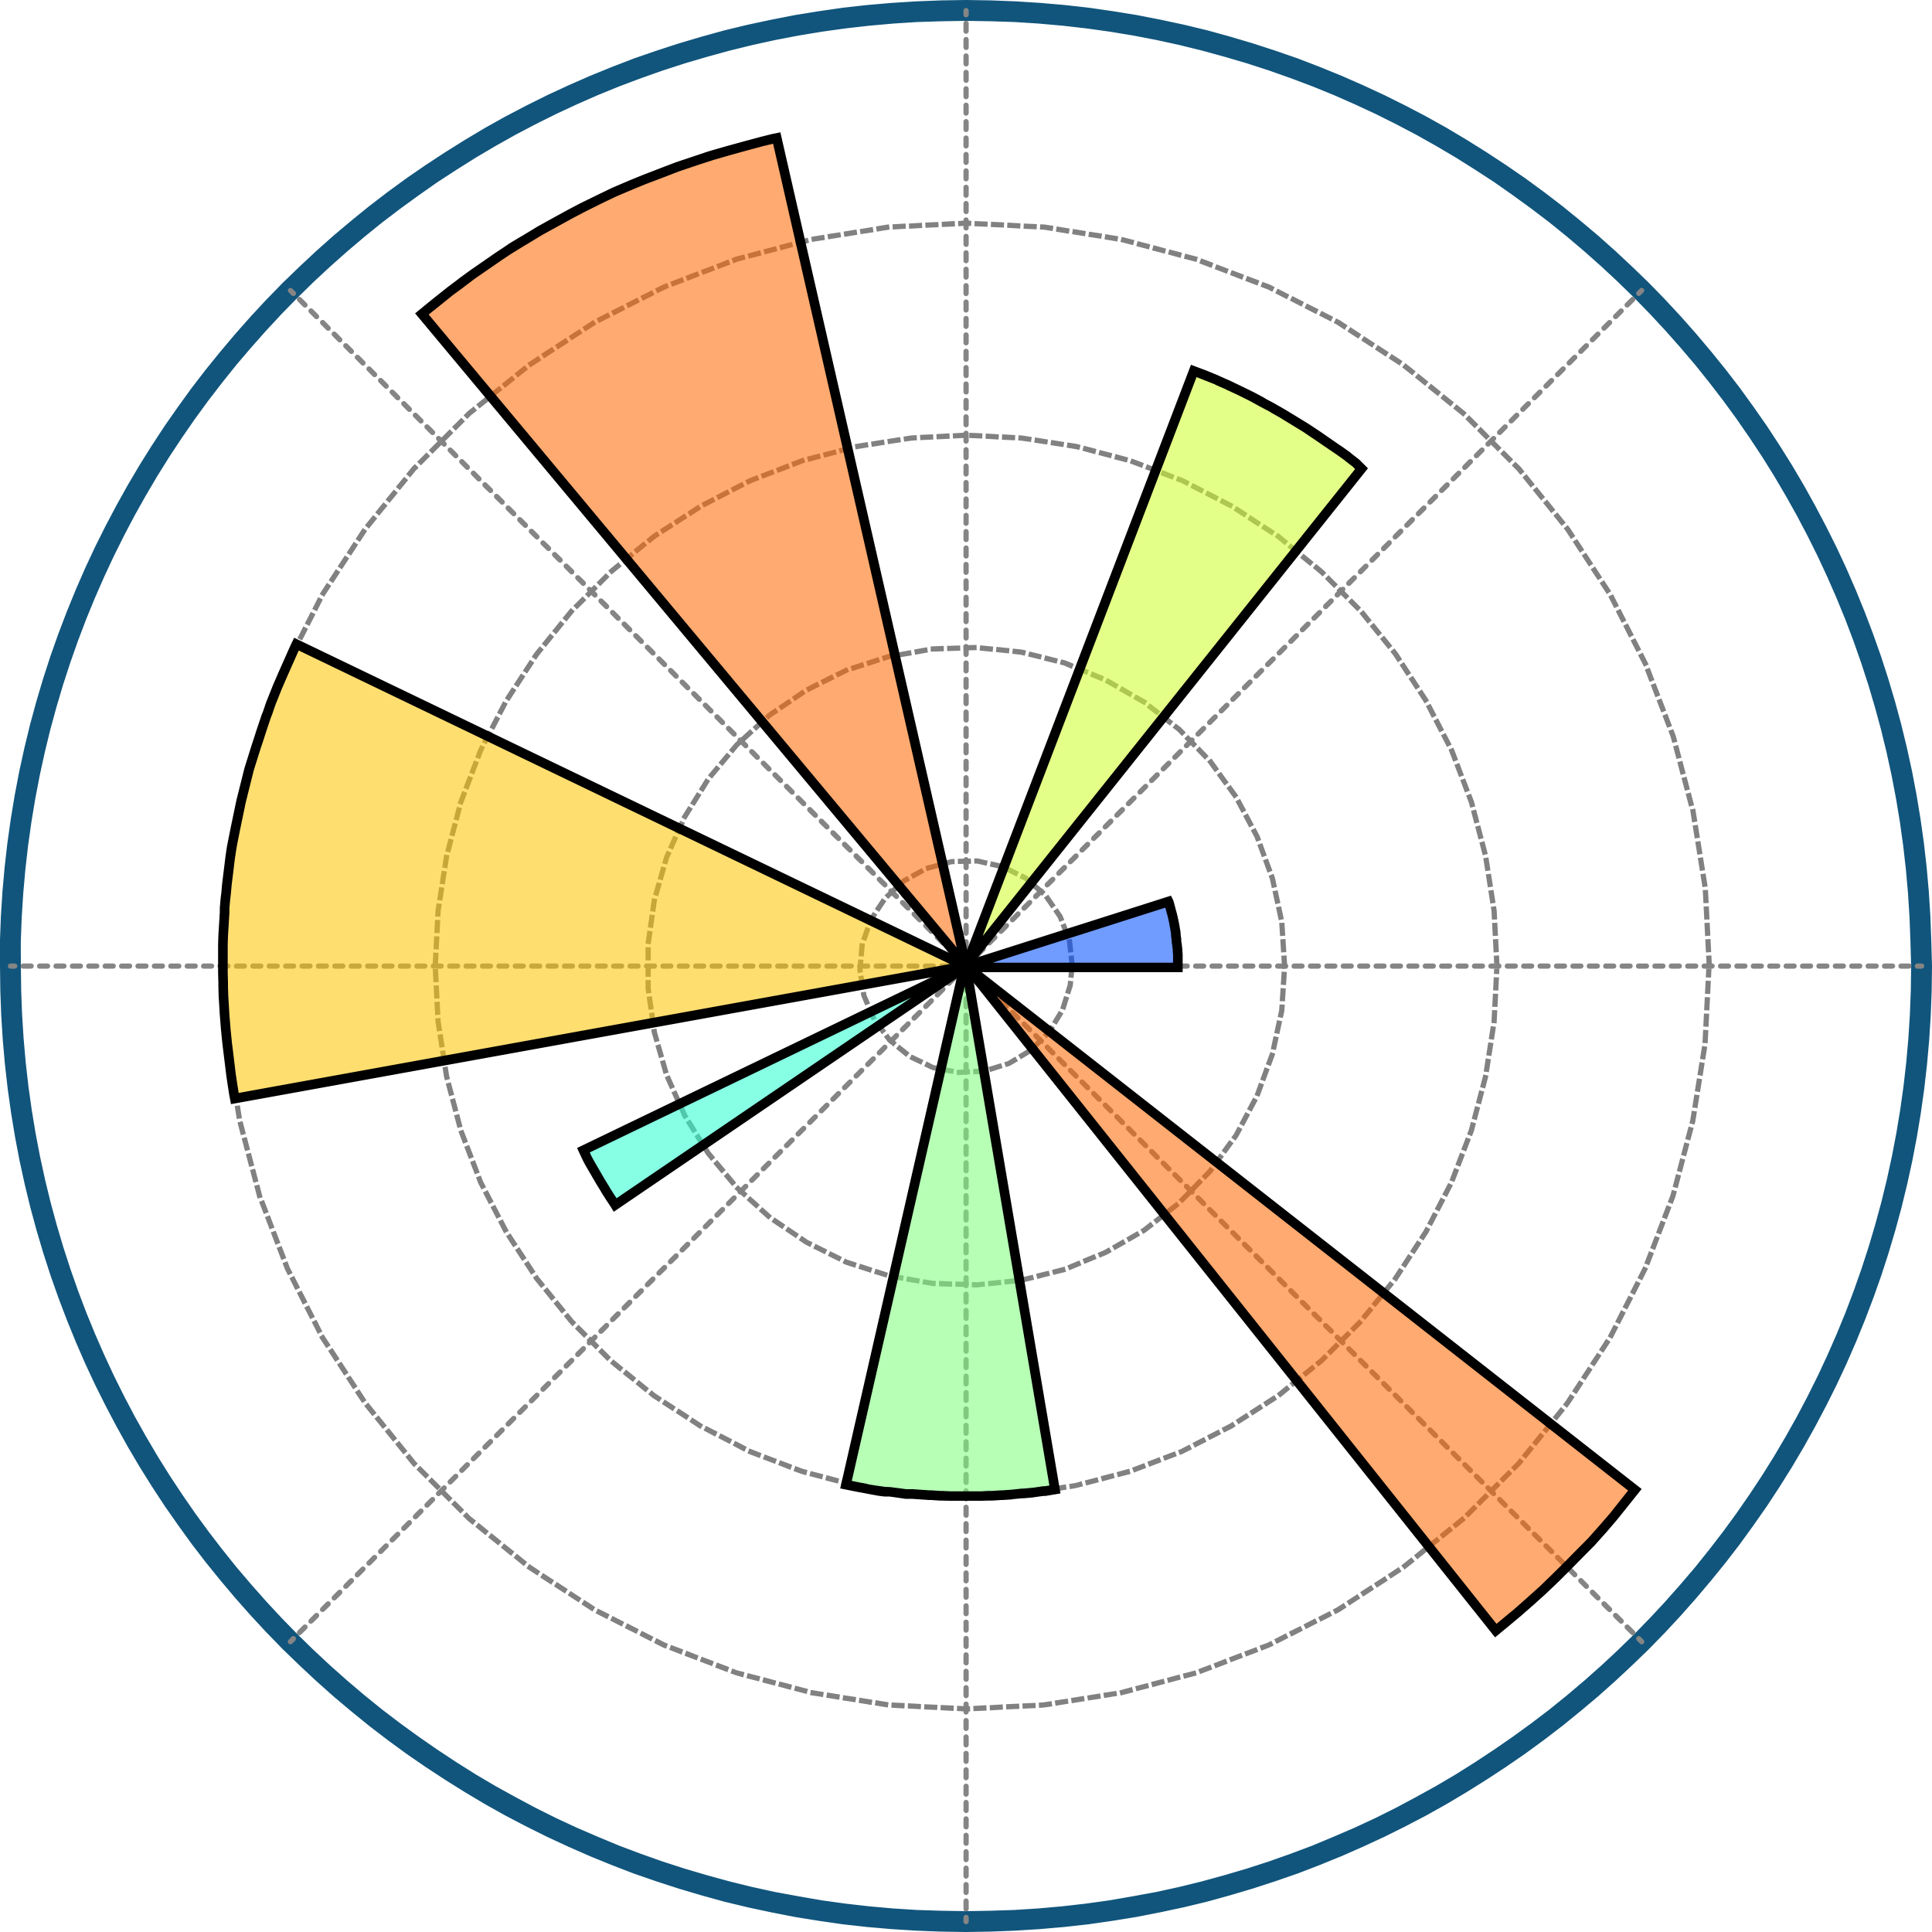
\includegraphics{img/marcoTeorico/matplotlib-logo.png}
                }
                \vspace{-0.25cm}
                \caption{\tiny~Logo de Matplotlib \textit{Adaptado de:}~\cite{Hunter:2007}}%
                \label{fig:Matplotlib_logo}
            \end{figure}
        \end{column}
    \end{columns}
\end{frame}

\begin{frame}{Biblioteca de GUI para Python}{PyQt}
    \begin{columns}
        \begin{column}{0.4\textwidth}
            % Aquí podrías incluir una imagen de ejemplo
            \centering
            \begin{figure}[H]
                \centering
                \adjustbox{max width=\textwidth, max height=0.5\textheight}{%
                
\includegraphics{img/marcoTeorico/qt-logo.png}
                }
                \vspace{-0.25cm}
                \caption{\tiny~Logo de PyQt.~\textit{Adaptado de:}~\cite{qt_wiki}}%
                \label{fig:PyQt_logo}
            \end{figure}
        \end{column}
        \begin{column}{0.6\textwidth}
            \begin{itemize}
                \item Basado en Qt (C++)
                \item Widgets y \textit{layouts}
                \item Integración con Matplotlib
                \item Soporte para multihilo
                \item Qt Designer
            \end{itemize}
        \end{column}
    \end{columns}
\end{frame}

\subsection[Métodos \& Técnicas]{Métodos \& Técnicas a utilizar.}

\begin{frame}{Cálculo de Gravedad y Colisiones}{Mediante módulos de \texttt{REBOUND}}
    \begin{columns}
        \begin{column}{0.6\textwidth}
            \small
            \begin{itemize}
                \item \textbf{Cálculo de Gravedad:}
                \begin{itemize}
                    \item \textbf{Suma Directa:} $O(N \cdot N_{\text{active}})$
                    \item \textbf{Octree (Barnes-Hut):} $O(N \log N)$
                \end{itemize}
                \item \textbf{Detección de Colisiones:}
                \begin{itemize}
                    \item \textbf{Búsqueda Directa:} $O(N^2)$
                    \item \textbf{Octree:} $O(N \log N)$
                    \item \textbf{Barrido Plano}
                \end{itemize}
            \end{itemize}
        \end{column}
        \begin{column}{0.4\textwidth}
            % Aquí podrías incluir una imagen de ejemplo
            \centering
            \begin{figure}[H]
                \centering
                \adjustbox{max width=\textwidth, max height=0.5\textheight}{%
                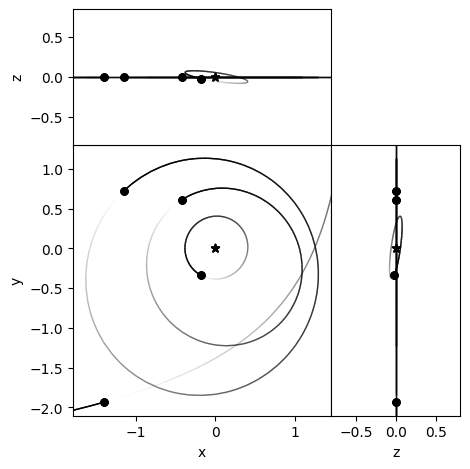
\includegraphics{img/marcoTeorico/rebound-simulation.png}
                }
                \vspace{-0.25cm}
                \caption{\tiny~Simulación de orbitas usando REBOUND \textit{Adaptado de:}~\cite{rebound_hyperbolic_orbits_2025}}%
                \label{fig:REBOUND_methods}
            \end{figure}
        \end{column}
    \end{columns}
\end{frame}

\begin{frame}{Algoritmo de Exploración}{Algoritmo Genético (AG) con pymoo}
    \begin{columns}
        \begin{column}{0.6\textwidth}
            \small
            \begin{itemize}
                \item \textbf{Componentes principales:}
                \begin{itemize}
                    \item \textbf{Muestreo}
                    \item \textbf{Selección de Padres}
                    \item \textbf{Cruce}
                    \item \textbf{Mutación}
                    \item \textbf{Manejo de Restricciones}
                \end{itemize}
            \end{itemize}
        \end{column}
        \begin{column}{0.4\textwidth}
            % Aquí podrías incluir una imagen de ejemplo
            \centering
            \begin{figure}[H]
                \centering
                \adjustbox{max width=\textwidth, max height=0.5\textheight}{%
                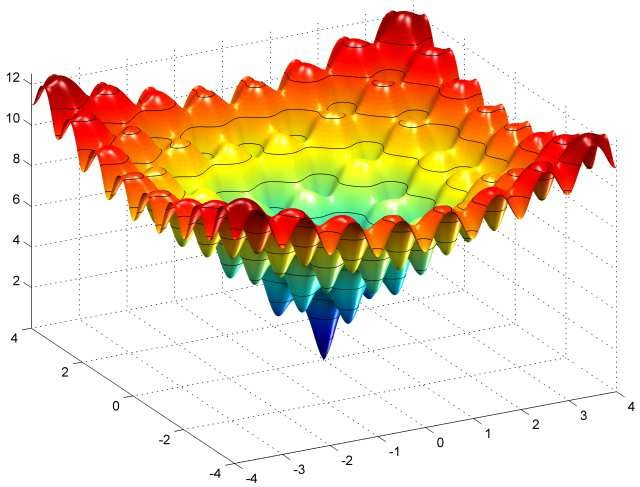
\includegraphics{img/marcoTeorico/benchmarkfunction.png}
                }
                \vspace{-0.25cm}
                \caption{\tiny~Funcion tipo benchmark, para la evaluación de AGs \textit{Adaptado de:}~\cite{silva2018}}%
                \label{fig:genetic_algorithm}
            \end{figure}
        \end{column}
    \end{columns}
\end{frame}

\begin{frame}{Indicador de Estabilidad}{Exponente de Lyapunov}
    \begin{columns}
        \begin{column}{0.4\textwidth}
            % Aquí podrías incluir una imagen de ejemplo
            \centering
            \begin{figure}[H]
                \centering
                \adjustbox{max width=\textwidth, max height=0.5\textheight}{%
                
\includegraphics{img/marcoTeorico/lyapunovExponent-in-randomAttractors.jpg}
                }
                \vspace{-0.25cm}
                \caption{\tiny~Atractor caótico generado mediante exponentes de Lyapunov.~\textit{Adaptado de:}~\cite{bourke_lyapunov_attractors_2001}}%
                \label{fig:Lyapunov_diagram}
            \end{figure}
        \end{column}
        \begin{column}{0.6\textwidth}
            \begin{itemize}
                \item Cuantifica sensibilidad
                \item Indicador primario de estabilidad/caos
                \item Medida objetiva y cuantitativa
                \item Predice comportamiento a largo plazo
                \item Base matemática rigurosa
            \end{itemize}
        \end{column}
    \end{columns}
\end{frame}

\begin{frame}{Enfoque del Proyecto}{Factibilidad y Optimización}
    \begin{columns}
        \begin{column}{0.4\textwidth}
            % Aquí podrías incluir una imagen de ejemplo
            \centering
            \begin{figure}[H]
                \centering
                \adjustbox{max width=\textwidth, max height=0.5\textheight}{%
                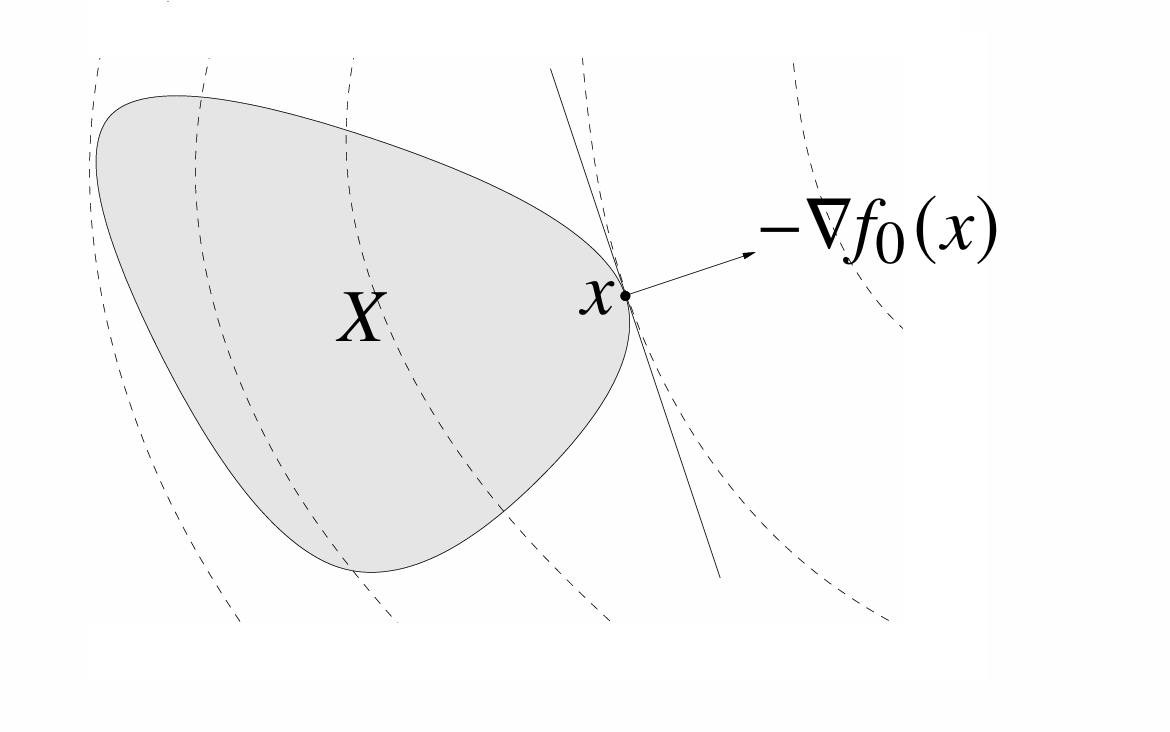
\includegraphics{img/marcoTeorico/optimizacion_fig1.png}
                }
                \vspace{-0.25cm}
                \caption{\tiny~Gráfica 2D que muestre contornos de una función objetivo $f_0(x)$,
                        una región factible sombreada definida por restricciones, y el punto óptimo $x^*$.\ \textit{Adaptado de:}~\cite{BoydVandenbergheSlides2023}}%
                \label{fig:factibility_optimization}
            \end{figure}
        \end{column}
        \begin{column}{0.6\textwidth}
            \small
            \begin{itemize}
                \item \textbf{Problema de Factibilidad:}
                \begin{itemize}
                    \item Determinar si existen configuraciones estables
                    \item Criterio clave: Exponente de Lyapunov $\lambda_1 \leq \text{umbral}$
                    \item Restricciones físicas. %masas positivas, parámetros orbitales válidos
                \end{itemize}
                \item \textbf{Marco de Optimización:} % (Herramienta)
                \begin{itemize}
                    \item Función objetivo: minimizar $\lambda_1$ directamente
                    \item Algoritmo Genético como herramienta exploratoria
                    \item Permite búsqueda eficiente en el espacio de parámetros
                \end{itemize}
            \end{itemize}
        \end{column}
    \end{columns}
\end{frame}
    \section{Planeación}
    \section{Análisis}

\begin{frame}{Matríz de procesos}
    \centering
    \captionof{table}{Matríz de procesos}
    \label{tab:procesos}
    \vspace{-0.1cm}
    \begin{adjustbox}{max width=0.9\textwidth,max height=0.7\textheight, keepaspectratio}
        \renewcommand{\arraystretch}{1.3}
            \begin{tabular}{@{}>{\bfseries}p{0.35\textwidth}  p{0.35\textwidth} p{0.35\textwidth}@{}}
            \toprule
            \textbf{Nombre del proceso} & \textbf{Objetivo} & \textbf{Salidas}  \\
            \midrule
            \textbf{Captura Parámetros} & Recopilar, validar y almacenar parámetros de configuración del usuario. & Estructura \texttt{\seqsplit{ConfigurationData}} validada, estado de UI actualizado. \\
            \midrule
            \textbf{Mostrar Resultados} & Presentar solución óptima y visualización final al usuario. & Actualización visual de la UI con resultados finales. \\
            \midrule
            \textbf{Evaluar Fitness} & Calcular fitness penalizado (\texttt{\seqsplit{F}\_p}) combinando LE y violaciones. & Valor numérico de $F_p(x)$. \\
            \midrule
            \textbf{Crear Nueva Simulación} & Instanciar un nuevo entorno de simulación vacío en \texttt{\seqsplit{REBOUND}}. & Referencia a nuevo objeto \texttt{\seqsplit{Simulation}}. \\
            \bottomrule
            \end{tabular}
    \end{adjustbox}
    \smallskip
\end{frame}


\begin{frame}{Matríz de procesos}
    \centering
    \captionof{table}{Matríz de procesos}
    \label{tab:procesos}
    \vspace{-0.1cm}
    \begin{adjustbox}{max width=0.9\textwidth,max height=0.7\textheight, keepaspectratio}
        \renewcommand{\arraystretch}{1.3}
            \begin{tabular}{@{}>{\bfseries}p{0.35\textwidth}  p{0.35\textwidth} p{0.35\textwidth}@{}}
            \toprule
            \textbf{Nombre del proceso} & \textbf{Objetivo} & \textbf{Salidas}  \\
            \midrule
            \textbf{Agregar Cuerpos} & Añadir una partícula con propiedades físicas a la simulación. & Instancia \texttt{\seqsplit{sim}} modificada con nueva partícula. \\
            \midrule
            \textbf{Iniciar/Ejecutar Simulación} & Ejecutar la integración numérica paso a paso hasta $T_{\max}$. & Estructura \texttt{\seqsplit{SimulationResult}} con trayectoria completa. \\
            \midrule
            \textbf{Recolectar Datos} & Extraer estado actual del sistema en instantes de visualización. & Estructura \texttt{\seqsplit{VisualizationState}} con instantánea del sistema. \\
            \midrule
            \textbf{Generar Gráficos} & Dibujar o actualizar la representación visual en la pantalla. & Representación gráfica actualizada en la UI. \\
            \bottomrule
            \end{tabular}
    \end{adjustbox}
    \smallskip
\end{frame}

\begin{frame}{Diccionario de Datos: Cuerpo celeste}
  \centering
  \captionof{table}{Cuerpo celeste.}
  \label{tab:diccionario_cuerpos_slide}
  \begin{adjustbox}{max width=0.9\textwidth}
    \begin{tabular}{@{}p{3cm} p{4cm} p{1.5cm} p{1.5cm} p{2.5cm}@{}}
      \toprule
      \textbf{Nombre del atributo} & \textbf{Descripción} & \textbf{Tipo} & \textbf{Rango} & \textbf{Ejemplo} \\
      \midrule
      \textbf{masa} & Masa del cuerpo celeste... & \texttt{float} & \(>0\) (positivos)... & 1.0 \\
      \midrule
      \textbf{a} & Semieje mayor de la órbita... & \texttt{float} & \(>0\) (positivos) & 1.0 \\
      \midrule
      \textbf{e} & Excentricidad orbital... & \texttt{float} & [0, 1) & 0.1 \\
      \midrule
      \textbf{inc\_deg} & Inclinación orbital... & \texttt{float} & [0°, 180°] & 30.0 \\
      \midrule
      \textbf{perturba} & Indica si se aplica... & \texttt{bool} & \texttt{True} o \texttt{False} & True \\
      \bottomrule
    \end{tabular}
  \end{adjustbox}
\end{frame}

\begin{frame}{Diccionario de Datos: Simulación}
  \centering
  \captionof{table}{Simulación.}
  \label{tab:diccionario_simulación_slide}
  \begin{adjustbox}{max width=0.9\textwidth}
    \begin{tabular}{@{}p{3cm} p{4cm} p{1.5cm} p{1.5cm} p{2.5cm}@{}}
      \toprule
      \textbf{Nombre del atributo} & \textbf{Descripción} & \textbf{Tipo} & \textbf{Rango} & \textbf{Ejemplo} \\
      \midrule
      \textbf{t\_max} & Tiempo total de simulación... & \texttt{float} & \( > 0 \) (positivos) & 100.0 \\
      \midrule
      \textbf{N\_steps} & Número de pasos a almacenar... & \texttt{entero} & \(>0\) (positivos) & 1000 \\
      \midrule
      \textbf{sim.units} & Unidades de la simulación... & \texttt{texto} & \texttt{AU, yr, Msun} & AU, yr, Msun \\
      \midrule
      \textbf{sim.integrator} & Indica el integrador numérico... & \texttt{texto} & \texttt{ias15, whfast, BS, mercurius} & ias15 \\
      \midrule
      \textbf{x, y, z} & Guarda las posiciones... & \texttt{array(float)} & \(>0\) (positivos) & [5.0, 230.0, 20.0] \\
      \bottomrule
    \end{tabular}
  \end{adjustbox}
\end{frame}

\begin{frame}{Diccionario de Datos: Métricas}
  \centering
  \captionof{table}{Métricas.}
  \label{tab:diccionario_métricas_slide}
  \begin{adjustbox}{max width=0.9\textwidth}
    \begin{tabular}{@{}p{3cm} p{4cm} p{2.5cm} p{1.5cm} p{2.5cm}@{}}
      \toprule
      \textbf{Nombre del atributo} & \textbf{Descripción} & \textbf{Tipo} & \textbf{Rango} & \textbf{Ejemplo} \\
      \midrule
      \textbf{times} & Array que guarda los tiempos... & \texttt{array(float)} & \(>0\) (positivos) & [0.0, 100.0, 200.0] \\
      \midrule
      \textbf{energy} & Energía total del sistema... & \texttt{float} & Valor real & -0.5 \\
      \midrule
      \textbf{a\_arr, a\_pert} & Array que guarda el semieje... & \texttt{array(float)} & \(>0\) (positivos) & [1.0, 1.5, 2.0] \\
      \midrule
      \textbf{e\_arr, e\_pert} & Array que guarda la excentricidad... & \texttt{array(float)} & [0, 1) & [0.1, 0.2, 0.3] \\
      \midrule
      \textbf{Exponente de Lyapunov ($\mathbf{\lambda}$)}& Indica la tasa de crecimiento... & \texttt{float} & Valor real & 0.01 \\
      \bottomrule
    \end{tabular}
  \end{adjustbox}
\end{frame}
    \section{Diseño}

    \section[Conclusiones]{Conclusiones y Trabajo a Futuro}

    \begin{frame}
        \begin{center}
            {\Huge\calligra~¡Gracias por su atención!}\\
            ¿Alguna pregunta o comentario?
        \end{center}
    \end{frame}

    \section*{Referencias}

    \begin{frame}[allowframebreaks]
        \frametitle{Referencias}
        \begingroup
        \fontsize{6pt}{7pt}\selectfont
        \printbibliography[heading=none]
        \endgroup
    \end{frame}

\end{document}